\chapter{Procesos de desarrollo}
\label{chap:procesos-desarrollo}

\par Un proceso de desarrollo en el mundo del software se define como:

\begin{quote}
\emph{El proceso de transformación de unos requerimientos en una solución. Un conjunto de pautas a seguir para completar el ciclo de vida de la solución de una manera organizada, sistemática y que ayude a las personas a completar los objetivos fijados}
\end{quote}

\par En SidelabCode Stack se optó por implementar el proceso de desarrollo de software \emph{iterativo e incremental} para crear el dise\~no de la forja SidelabCode Stack a través de metodolog\'ias ágiles.

\par El proceso de desarrollo infiere directamente en la calidad del software que se construye. Es la parte más importante en el software ya que un proceso de desarrollo óptimo para una solución otorga las herramientas necesarias para una mejor evolución del mismo. Cada proceso de desarrollo ha de aplicarse a la solución según los requisitos de la misma, no todos los procesos de desarrollo son válidos para todos los proyectos.

\section{Software de Calidad}
\label{sec:software-calidad}

\par Desarrollar Software de Calidad, para ellos nos encontramos con la palabra \emph{"Calidad"} tan subjetiva en muchos ámbitos, pero que en el desarrollo puede ser bastante objetiva ya que se trata de Software, una ciencia evaluable. La Calidad del Software es el conjunto de cualidades que lo caracterizan y determinan su viabilidad y utilidad; Mantenibilidad, Fiable, Eficiencia y Seguridad.

\begin{figure}[H]
    \begin{center}	
        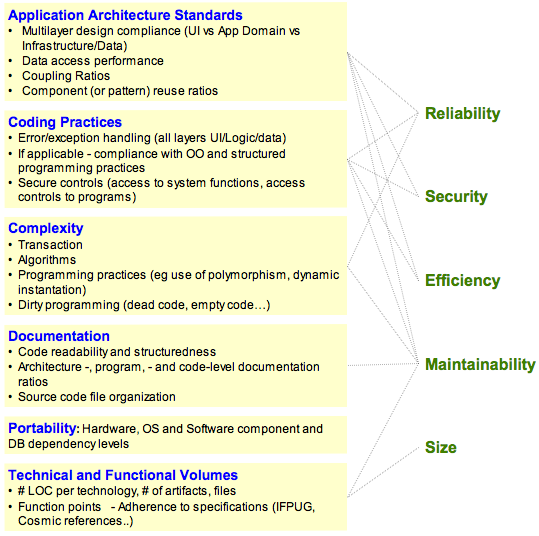
\includegraphics[width=0.9\textwidth]{SoftwareQuality}
        \caption{Software de Calidad}
        \label{fig:softwarequality}
    \end{center}
\end{figure}

\par Un software hecho para ejecutarse una sola vez no requiere el mismo nivel de calidad mientras que un software para ser explotado durante un largo necesita ser fiable, seguro, mantenible y flexible para disminuir los costes.

\begin{itemize}
	\item \emph{Mantenibilidad}: El software debe ser diseñado de tal manera, que permita ajustarlo a los cambios en los requerimientos. Esta característica es crucial, debido al inevitable cambio del contexto en el que se desempeña un software.
	\item \emph{Fiabilidad}: Incluye varias características además de la fiabilidad, como la aplicación de estándares, complejidad, tratamiento de errores.
	\item \emph{Eficiencia}: Tiene que ver con el uso eficiente de los recursos que necesita un sistema para su funcionamiento.
	\item \emph{Seguridad}: La evaluación de la seguridad requiere un control sobre la arquitectura, el diseño y las buenas prácticas.
\end{itemize}

% section software-calidad (end)

\section{Proceso iterativo}
\label{sec:proc-iterativo}

\par ¿ Que es el proceso iterativo ?

\begin{quote}
    \emph{La primera versión debe contener todos los requerimientos del usuario y lo que se va a hacer en las siguientes versiones es ir mejorando aspectos como la funcionalidad o el tiempo de respuesta.}\footnote{Procesos Iterativos e Incrementales - \url{http://esalas334.blogspot.es/1193761920/}}
\end{quote}

\par Se centra más en la inmediatez de la primera versión y en las mejoras posteriores que se van creando enfocadas a la solución final. En el proceso también juega una parte fundamental la comunicación con el cliente a través de la visualización de los resultados por iteraciones. De esta forma se consigue una buena coordinación entre el cliente y el equipo de desarrollo para la consecución de los objetivos.

\begin{figure}[H]
    \centering
    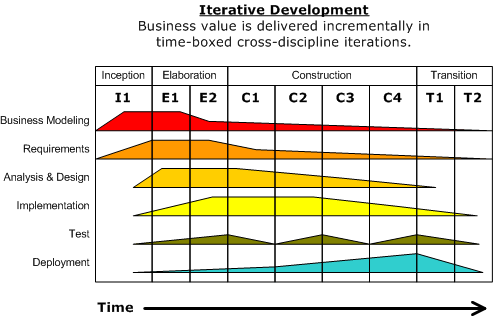
\includegraphics[width=0.9\textwidth]{DevelopmentIterative}
    \caption{Desarrollo Iterativo}
    \label{fig:desarrollo-iterativo}
\end{figure}

\par Se han de tener en cuenta posibles cambios entre iteraciones pero nunca del resultado completo, para que de esta forma se pueda controlar a tiempo la \emph{desviación} que pueda existir en el proceso de la creación de producto.

\begin{quote}
    \emph{Como la idea que representa la palabra iterativo, un proceso de desarrollo de software iterativo es aquel al que se lo piensa, como una serie de tareas agrupadas en pequeñas etapas repetitivas. Estas "pequeñas etapas repetitivas" son las iteraciones.}\footnote{Proceso de Desarrollo Iterativo - Fernando Soriano - \url{http://fernandosoriano.com.ar/?p=13}}
\end{quote}

\par La base el proceso de desarrollo Iterativo provee un conjunto de pasos para el desarrollo de la solución que se repiten iteración tras iteración para la creación de mejoras tangibles y/o evaluables. 

\begin{figure}[H]
    \centering
    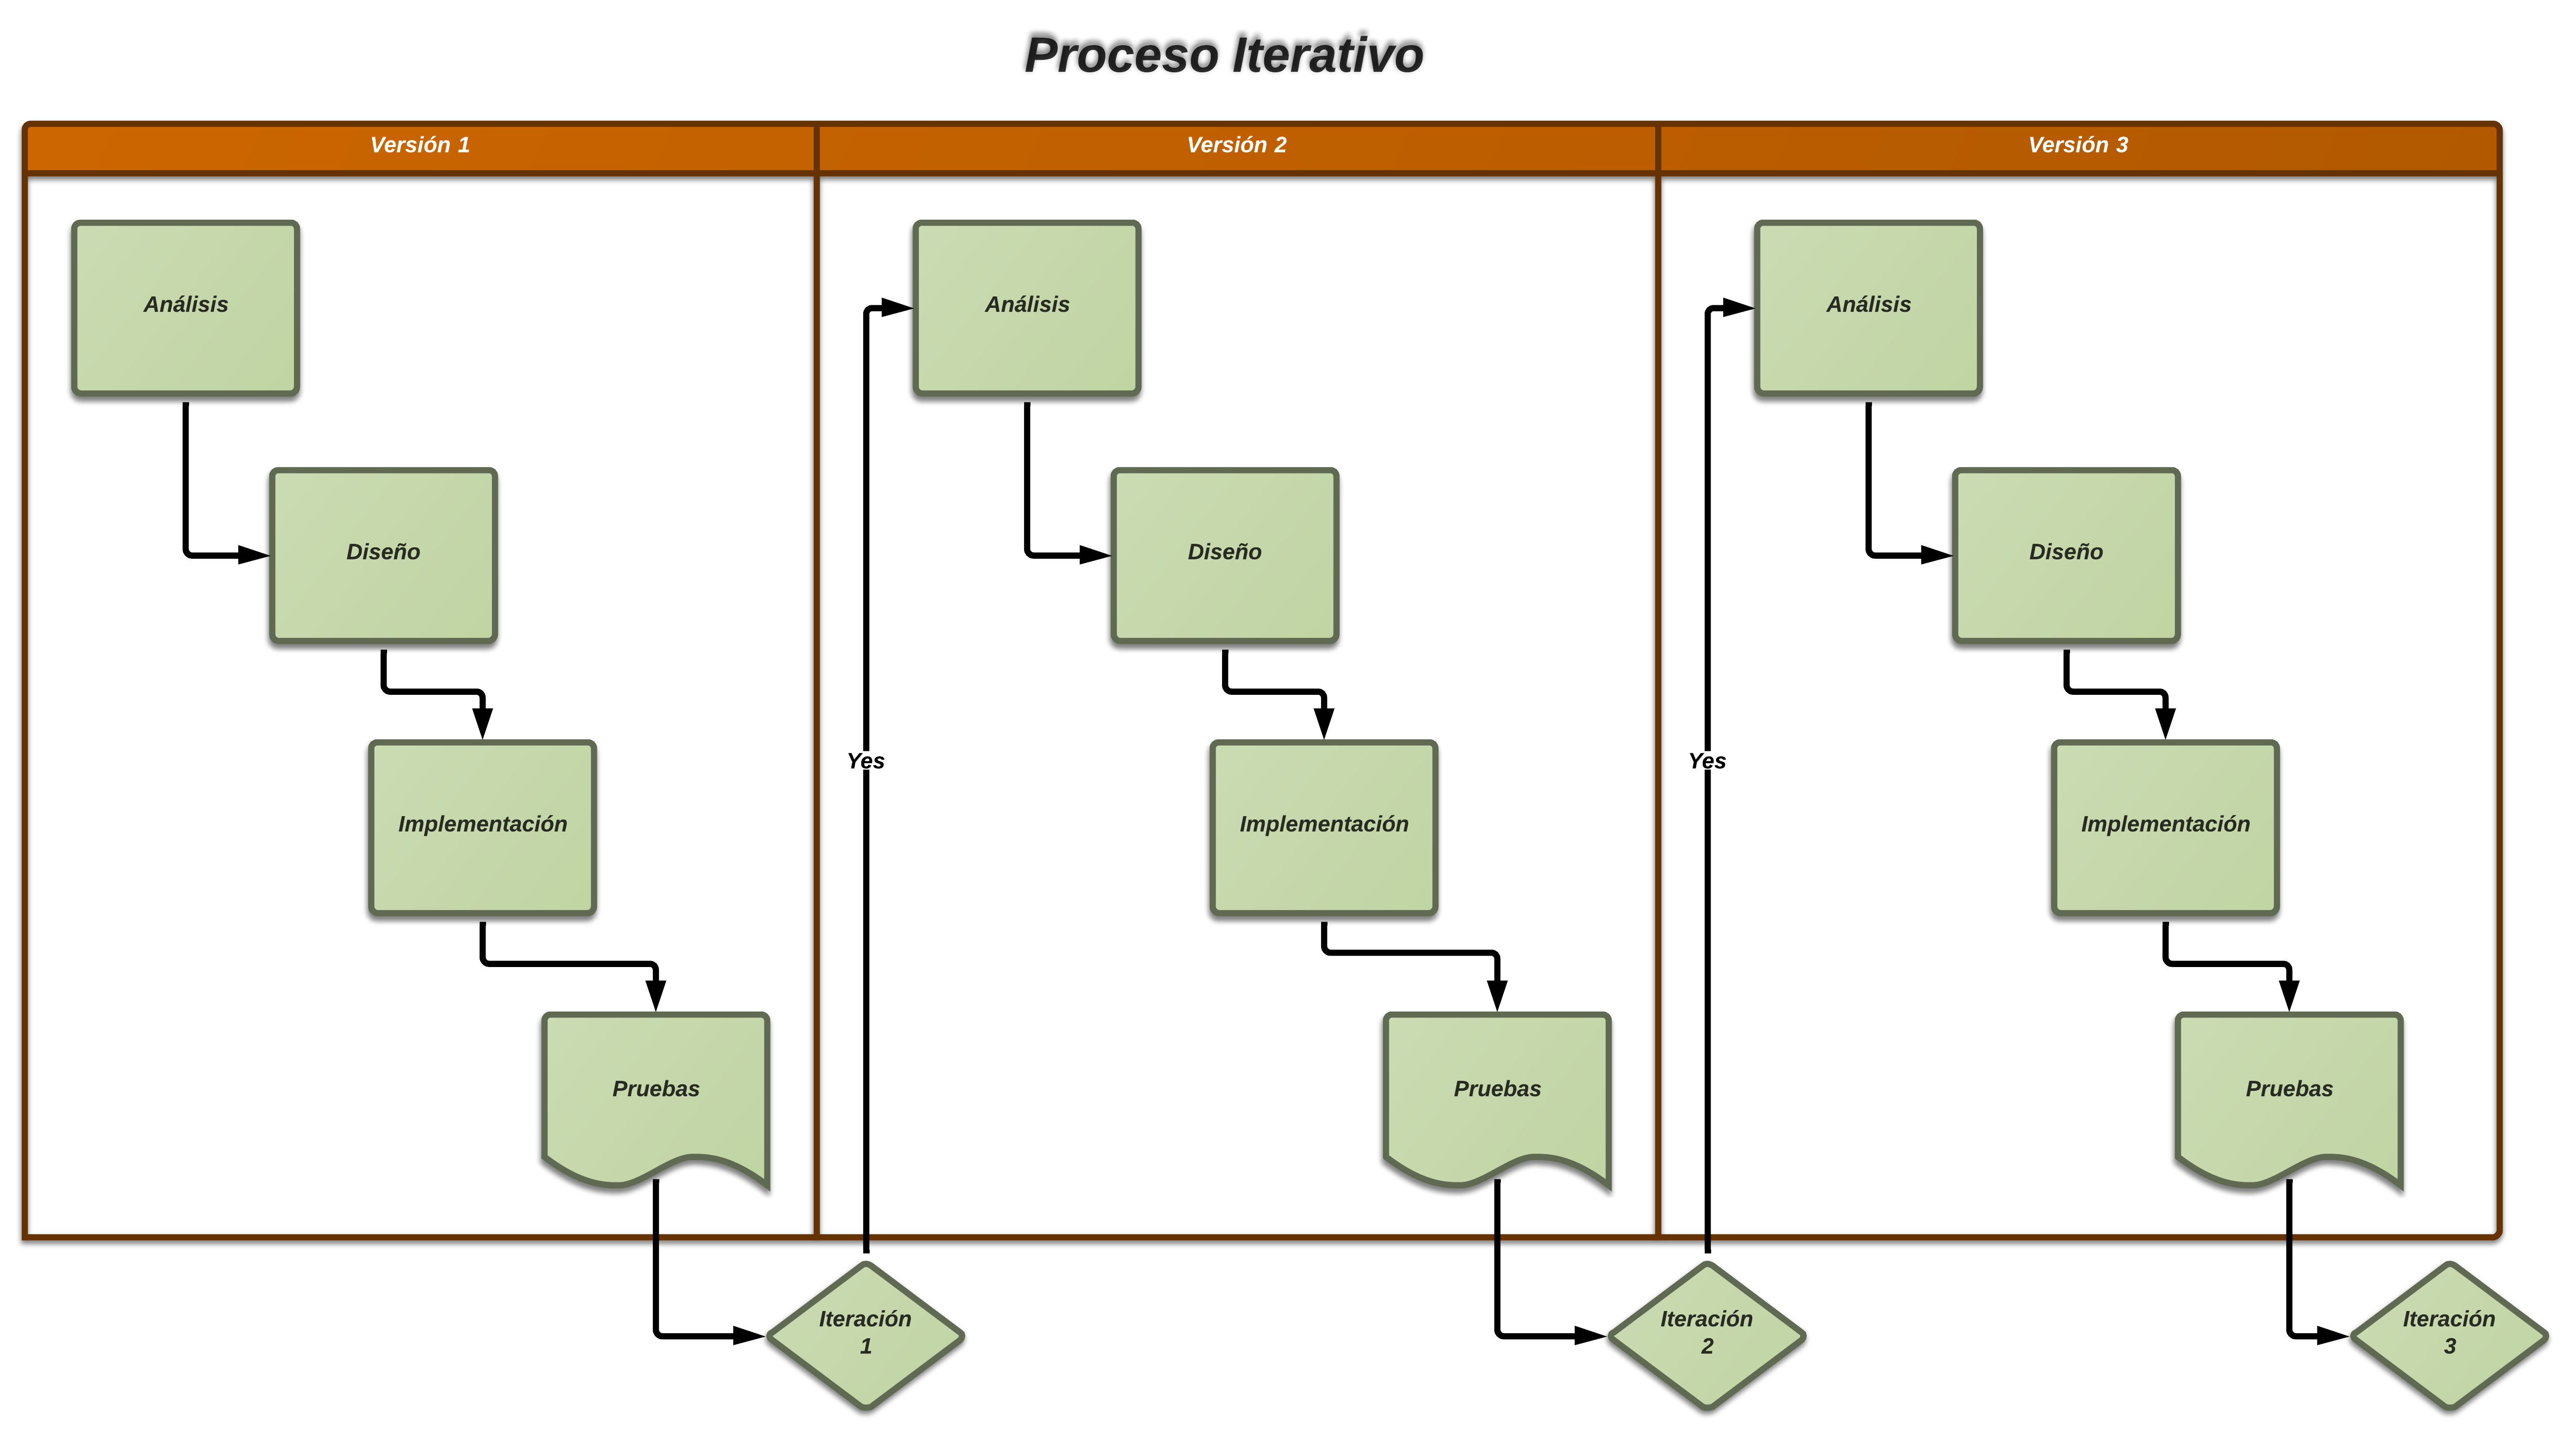
\includegraphics[width=0.9\textwidth]{ProcesoIterativo}
    \caption{Proceso Iterativo}
    \label{fig:ProcesoIterativo}
\end{figure}

\par En cada iteración se construye una pieza funcional del producto final, completa, testeada, documentada e integrada en la solución final. La visión completa de este proceso muestra una línea de iteraciones separadas funcionalmente unas de otras que en conjunto, forman la solución final. Iteraciones independientes unas de otras a través de un desarrollo lineal agrupando pequeños ciclos de desarrollo.

\begin{itemize}
	\item \emph{Duración fija}, quiere decir que una vez establecidos los tiempos o planificación de la iteración, la iteración termina en la fecha exacta establecida. Si el equipo no pudo cumplir lo planificado, el desarrollo pendiente pasa a otra iteración.
	\item Estimación de tiempos cortos, las \emph{"buenas prácticas"} hablan de que una iteración debiera durar entre 2 y 6 semanas.
	\item Es como un ciclo de desarrollo completo, ya que en una iteración se realizan actividades de análisis, diseño, implementación, pruebas, etc.
\end{itemize}

% section proc-iterativo (end)

\section{Proceso incremental}
\label{sec:proc-incremental}

\par El Proceso Incremental fue propuesto por \emph{Harlan D. Mills} en 1980.

\par Sugirió el enfoque incremental de desarrollo como una forma de reducir la repetición del trabajo en el proceso de desarrollo y dar oportunidad de retrasar la toma de decisiones en los requisitos hasta adquirir experiencia con el sistema.

\par El modelo incremental combina elementos del modelo lineal secuencial (aplicados repetidamente) con la filosofía interactiva de construcción de prototipos. El modelo incremental aplica secuencias lineales de forma escalonada mientras progresa el tiempo en el calendario.

\par Cada secuencia lineal produce un \emph{"incremento"} en el desarrollo de la solución. Por ejemplo, en relación a la forja SidelabCode Stack; en la primera versión estaba accesible el módulo de Jenkins, en el siguiente incremento la configuración de Jenkins se ligaba automáticamente a la configuración del los usuarios por proyecto, el siguiente incremento se publicaban las instrucciones para gestionar Jenkins a partir de una cuenta y facilitar la configuración para los distintos entornos.

\begin{figure}[H]
    \centering
    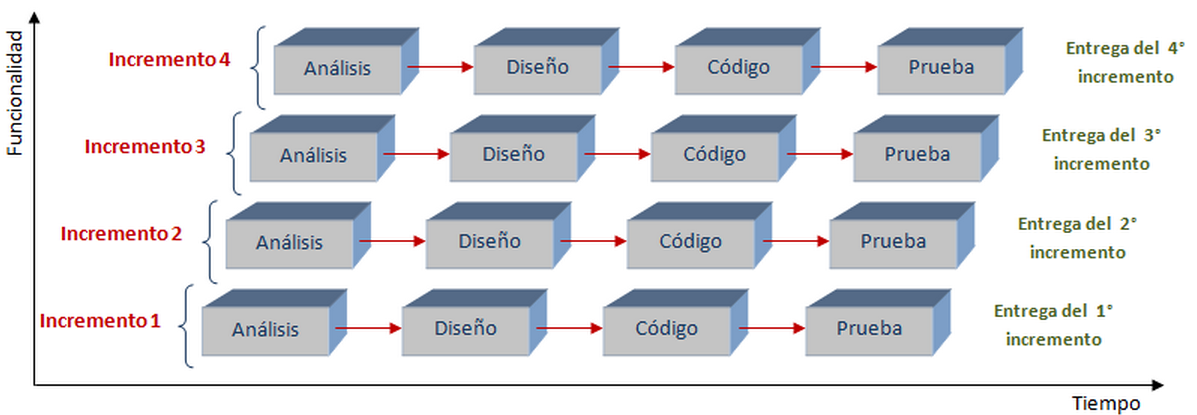
\includegraphics[width=0.9\textwidth]{modelo_incremental}
    \caption{Modelo Incremental}
    \label{fig:modelo-incremental}
\end{figure}

\par Al iniciar el desarrollo, los clientes o los usuarios, identifican a grandes rasgos las funcionalidades que proporcionará el sistema. Se define un bosquejo de requisitos funcionales y será el cliente quien se encarga de priorizar que funcionalidades son más importantes. Con las prioridades definidas, se puede confeccionar el plan de incrementos, en donde cada incremento se compone de un subconjunto de funcionalidades a desarrollar.

% section proc-incremental (end)

\section{Iterativo e Incremental}
\label{sec:iterativo-incremental}

\par Desarrollo iterativo e incremental. La conjunción de estos dos tipos de desarrollo aúnan las mejores cualidades de ambos para gestión de un equipo de trabajo en la construcción de una solución.

\par El proceso iterativo e incremental se basa en incrementos por cada una de las iteraciones en el proceso de desarrollo. La idea básica de este proceso es desarrollar una solución a través de las iteraciones de ciclos a partir de los incrementos en la funcionalidad para que los desarrolladores mejoren su productividad en torno al proyecto a partir de pequeños hitos que completan versiones usables de la solución desde la primera implementación.

\begin{figure}[H]
    \centering
    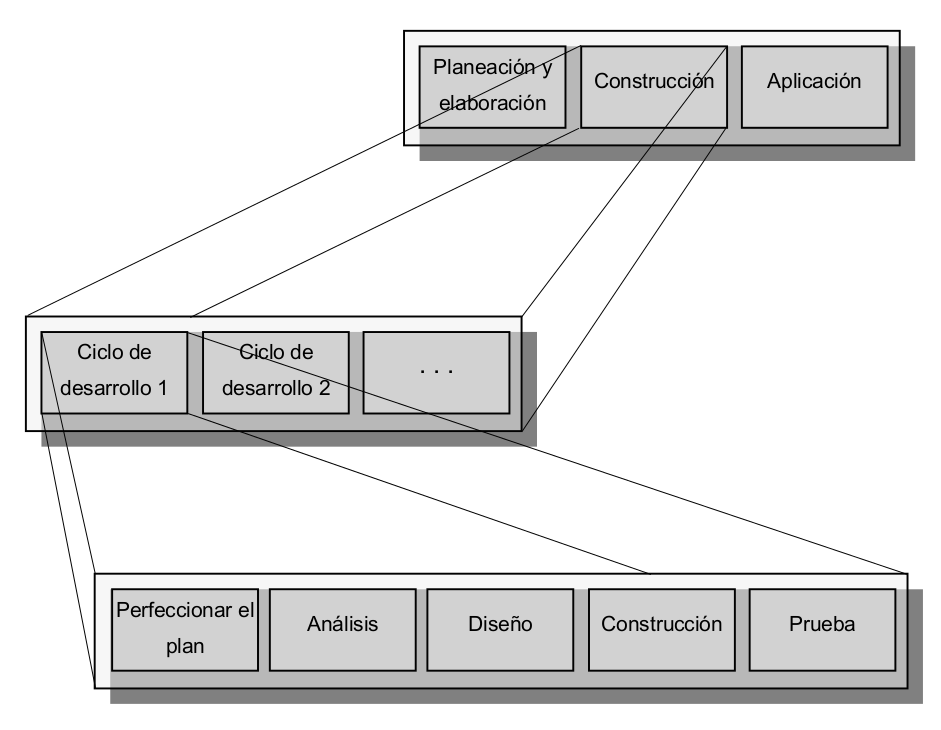
\includegraphics[width=0.9\textwidth]{iterativo-incremental-larman}
    \caption{Proceso iterativo e Incremental por Larman}
    \label{fig:iterativo-incremental-larman}
\end{figure}

\par La evolución de la solución se basa en las iteraciones pasadas añadiendo los nuevos requisitos/objetivos (pueden ser mejoras o nuevas funcionalidades). Se basa en incrementar el valor del trabajo hecho para tener un control del proceso más exhaustivo priorizando los objetivos. Por cada iteración existen modificaciones en el diseño y en las funcionalidades.

\par La comunicación y la implicación en el desarrollo del proyecto con el usuario/cliente desde el inicio del proyecto es crucial ya que el proceso parte desde una solución inicial para incluir versiones usables con el usuario/cliente. De esta forma todas las partes aportan sus distintos puntos de vista de una manera continua implicándose en el proceso y midiendo el crecimiento de la solución paso a paso, incremento a incremento.

\par Este proceso de desarrollo cercano a las \emph{Metodologías Ágiles}, como ellas tiene el mismo fin, la implicación, desarrollo, fiabilidad, confianza, aprendizaje, versatilidad, responsabilidad, comunicación con la solución desarrollada y el usuario/cliente durante el proceso.

\par Una de las claves en este proceso es la retroalimentación y el aprendizaje del grupo de trabajo a partir de las iteraciones. De esta forma el trabajo hecho repercute en las iteraciones futuras aportando nuevos conocimientos sobre el proceso y el desarrollo. Creando mejores iteraciones y evoluciones de la solución, \emph{profesionalizando el trabajo}.

\par Las Iteraciones han de ser de una duración corta de \emph{2 a 6 semanas} para que la comunicación a todos los niveles del proyecto siga siendo fluida y para que si en algún caso se haya de desechar una Iteración no se pierda mucho trabajo desarrollado en ella. Esto no ocurre muy a menudo pero se contempla por diferentes causas:

\begin{itemize}
	\item Abandono del proyecto.
	\item Cambio de Cliente/Usuario.
	\item Falta de recursos.
\end{itemize}

\par Las Iteraciones \emph{"cortas"} otorgan al modelo un alto nivel de versatilidad a la hora de evolucionar y evaluar el recorrido del trabajo hecho en el proyecto, para así poder predecir la organización de las futuras iteraciones.

\subsection{Fases del proceso}
\label{sub:fases-proceso}

\par El proceso de desarrollo Iterativo e Incremental está basado en tres fases:

\begin{itemize}
	\item Iniciación.
	\item Iteración.
	\item Lista del Control del Proyecto.
\end{itemize}

\par El objetivo de la \emph{Iniciación} es la implementación inicial para crear un producto con el cual el usuario/cliente pueda interactuar y tener las primeras impresiones. El equipo de desarrollo y el usuario/cliente toman como punto base esta fase de \emph{Iniciación}.

\par Esta primera implementación ha de servir de guía para la evolución del desarrollo en cada una de las iteraciones, la base.

\par La \emph{Lista de Control del Proyecto} es el lugar donde se definen las tareas que han de cumplimentarse durante el proceso de desarrollo. Todos los aspectos relacionados con la implementación de la solución se encuentran definidos en la lista, funcionalidades, diseño, errores, mejoras. La Lista de Control está en constante evolución, no es un muro estático, ya que se van adjuntando las funcionalidades y/o mejoras y posibles nuevas funcionalidades. De esta forma se evalúan las prioridades en la fase de análisis por cada iteración y se decide que tareas han de implementarse y cuales son desechadas para la siguiente iteración.

\par La \emph{Iteración} es un conjunto modular de acciones a llevar a cabo para cumplir con las tareas que se definen para evolucionar la solución por incrementos. Debe estar sujeta a cambios en el diseño, nuevas tareas añadidas a la lista de control y sobretodo, ser simple.

% subsection fases-proceso (end)

\subsection{Desarrollo Iteración}
\label{sub:desarrollo-iteracion}

\par El desarrollo del proyecto viene medido por las Iteraciones que se conectan una a otra secuencialmente.

\par La iteración comienza a partir del análisis basado en la retroalimentación de los usuarios y los servicios de análisis disponibles. Los elementos a tener en cuenta en el análisis son:

\begin{itemize}
	\item Estructura.
	\item Modularidad.
	\item Ergonomía.
	\item Eficiencia.
	\item Objetivos logrados.
\end{itemize}

\par Se han tener en cuenta los posibles riesgos que puedan surgir en la Iteración para evaluarlos y eliminarlos en el momento de definir la línea base de la arquitectura. Además el equipo de desarrollo ha de dominar y estar al tanto del lenguaje empleado en los requisitos, el problema que se va a abordar y de esta manera ser capaces de asumir los posibles riesgos o imprevistos que puedan surgir.

\par Los resultados del análisis se reflejan en la Lista de Control del proyecto para añadir, modificar y ordenar por prioridades para la siguiente Iteración.

\par En las Iteraciones posteriores ha de aumentar la capacidad de reducir los riesgos, desarrollar los componentes e ir evolucionando incremento a incremento hacia la versión final para el usuario/cliente.

\par Cada Iteración se reduce a un \emph{miniproyecto} (Se les llama miniproyectos porque no es algo que el usuario haya pedido) que consta del proceso de requisitos, análisis, diseño, implementación y prueba.

\begin{figure}[H]
    \centering
    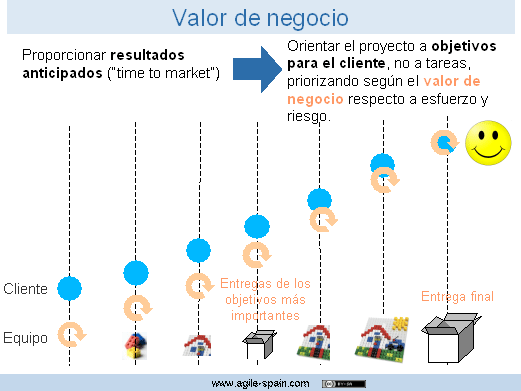
\includegraphics[width=0.9\textwidth]{valor-negocio-iterativo-incremental}
    \caption{Valor de negocio Iterativo e Incremental}
    \label{fig:valor-negocio-iterativo-incremental}
\end{figure}

\par El proceso de desarrollo en una Iteración se reduce a una serie de guías o pasos a seguir en torno a las modificaciones que surgen a la medida que se avanza en el desarrollo. El proceso Iterativo e Incremental se basa en la flexibilidad por lo tanto las modificaciones de la Iteración han de ser otra herramienta más para lograr los objetivos y como tales:

\begin{itemize}
	\item Cualquier dificultad encontrada en el diseño, desarrollo y prueba de una modificación puede alertar de la necesidad de cambiar el diseño o la implementación. Se han de desarrollar las modificaciones con una estructura modular y aislada (en su medida) para poder trabajar en un problema o solución concreta y que no afecte al resto de la implementación.
	\item Las modificaciones han de ser sencillas de implementar, sino se ha de rediseñar el la solución.
	\item Las modificaciones han de ser más sencillas conforme se van completando iteraciones. Si esto no ocurre existe un problema de diseño y puede incurrir en el exceso de soluciones \emph{ad-hoc}, parches.
	\item Los parches se contemplan como soluciones temporales en distintas iteraciones para que no sea necesario un cambio en el diseño, pero sólo para casos excepcionales. Si los parches proliferan se ha de replantear el diseño.
	\item La implementación existente ha de ser analizada constantemente para certificar que sigue el camino marcado por los objetivos a corto y largo plazo del proyecto. De esta forma se controlan las posibles desviaciones de tiempo y el trabajo hecho por el grupo de trabajo.
	\item Los herramientas de análisis se han de utilizar para validad los análisis y/o funcionalidades de las implementaciones parciales de la solución.
	\item La participación del usuario/cliente en el proceso ha de ser solicitada y analizada para contemplar posibles deficiencias o errores en la implementación actual. De esta forma es como se ha de crear una canal de comunicación para interactuar con el grupo de trabajo.
\end{itemize}

% subsection desarrollo-iteracion (end)


% section iterativo-incremental (end)
\section{Gestión de tareas}
\label{sec:gestion-tareas}

\par¿ Qué hay que hacer ? ¿ Quién tiene que hacerlo ? ¿ Cuando hay que hacerlo ?

\par \emph{David Allen} propulsor de la metodología \emph{GTD} (Getting Things Done):

\begin{quote}
    \emph{El método GTD se basa en la idea de trasladar las tareas y los proyectos previstos de la mente mediante el registro de forma externa y luego dividiéndolos en los elementos de trabajo viables. Esto permite centrar la atención en la adopción de medidas en las tareas, en lugar de en recordarlos}
\end{quote}

\par La organización centra la parte más importante en el desarrollo Iterativo e Incremental. Es el apartado donde se ha de dedicar más esfuerzo pero en donde se reciben mejores recompensas al trabajo bien hecho. Cuanto mejor se organiza la información con respecto al proceso, más y mejor crece la capacidad de afrontar nuevas iteraciones en el grupo de trabajo partiendo de la información generada a través del mismo.

\par En este apartado se introduce el concepto de \emph{Gestión de Tareas} para una óptima organización. Un gestor de tareas no es otra cosa que una agenda. Limitándonos a la definición de la \emph{RAE} (Real Academia de la lengua Española):

\begin{quote}
    \emph{"Libro o cuaderno en que se apunta, para no olvidarlo, aquello que se ha de hacer."}
\end{quote}

\par Una agenda es la herramienta que permite apuntar los trabajos, citas, recordatorios, listas de la compra para organizarlos según un orden de prioridad en base a las necesidades y el tiempo.

\par El Gestor de Tareas nos permite \textbf{organizar} las tareas que se han de hacer con respecto al proyecto. Es la herramienta que contiene la \emph{Lista de Control del Proyecto} y la gestiona con respecto a cada iteración para adjuntar las tareas y repartirlas entre los miembros del grupo de trabajo.

\par El gestor de tareas va un nivel más allá y dota de vida a las tareas creando un seguimiento:

\begin{itemize}
	\item Añadiendo información. En que se basa cada tarea.
	\item Cambios de encargados de las tareas. Pueden pasar de un usuario a otro.
	\item Ciclo de vida de las tareas. Desde que se crea hasta que se finaliza (diferentes motivos).
	\item Evaluar la prioridad. Dando un peso específico a cada una de las tareas dentro del proyecto.
	\item Visibilidad a todo el grupo de trabajo. Todo el mundo puede acceder a la información dependiente de cada tareas.
	\item Permite la planificación de la iteración. Desde el nivel más bajo al más alto se puede hacer un seguimiento minucioso del estado del proyecto.
\end{itemize}

\par La gestión de la tareas depende de todo el grupo de trabajo, desde el cliente (Lista de Control), el encargado de definir las iteraciones (Obteniendo las tareas de la Lista de Control) y el grupo de desarrolladores (Gestionando las tareas conforme avanza su trabajo). En cada uno de los estados se ha de hacer una planificación de cada una de las tareas y a cada iteración de la solución la planificación será mejor con respecto a la anterior, ya que el histórico ayuda a aprender del trabajo hecho hasta la fecha.

\par Como características principales de un Gestor de Tareas podemos definir:

\begin{itemize}
	\item Gestión de recursos.
	\item Gestión de tiempo.
	\item Gestión de iteraciones.
	\item Histórico de información.
\end{itemize}

% section gestion-tareas (end)

\section{Código versionado}
\label{sec:codigo-versionado}

\par Código versionado -> repositorios de código

% section codigo-versionado (end)

\section{TDD y CI}
\label{sec:tdd-ci}

\par TDD -> sistemas de CI para asegurar que los tests se pasan regularmente

% section tdd-ci (end)

\section{Desarrollo por canales}
\label{sec:desarrollo-canales}

% section desarrollo-canales (end)

\section{Herramientas}
\label{sec:herramientas}

% section herramientas (end)
